\section{Algorithmes de Dijkstra et A*}


\paragraph{Algorithme de Dijkstra : }Edgser Wybe Dijkstra, physicien néerlandais reconverti à l'informatique en 1955, a proposé en 1959 un algorithme de recherche de chemin minimum dans un graphe.

\begin{figure}[htp]
  \centering
  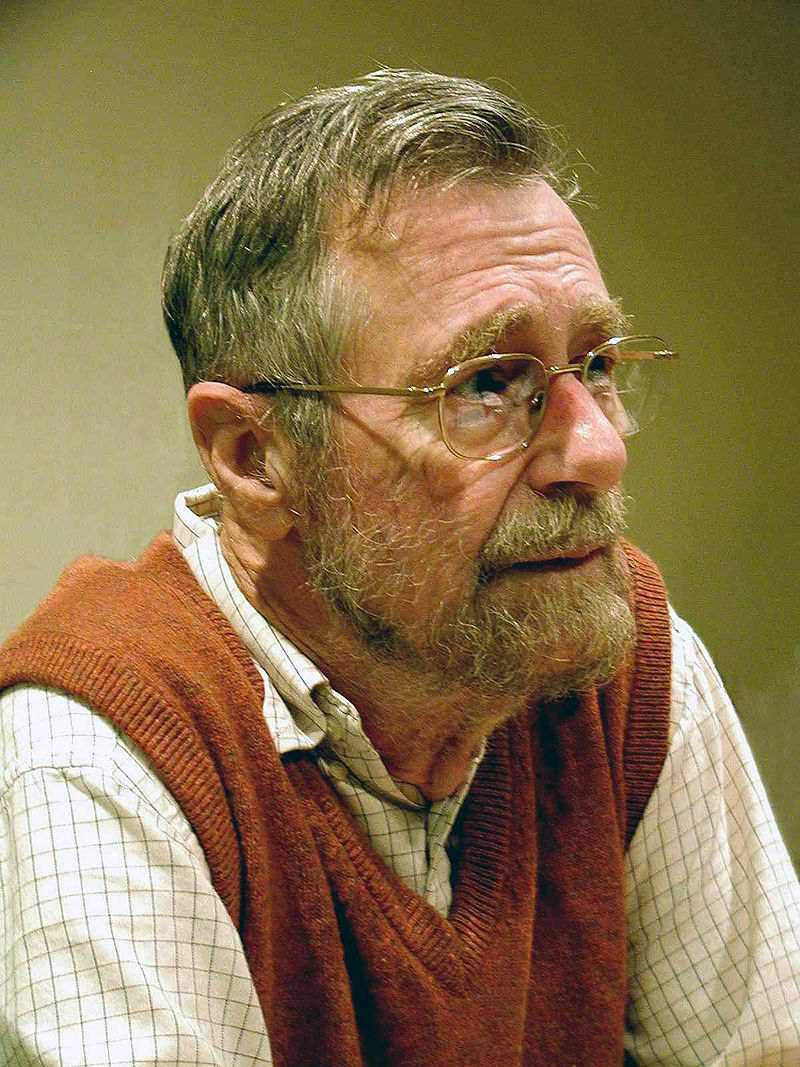
\includegraphics[width=4cm]{images/Edsger_Wybe_Dijkstra}
  \caption{Edgser Wybe Dijkstra (1930-2002)}
  \label{fig:une-autre-image}
\end{figure}

On doit à Dijkstra, qui avait la réputation d'avoir mauvais caractère et qui était notoirement allergique au ``GOTO'',
quelques citations\footnote{Source : \url{https://fr.wikipedia.org/wiki/Edsger_Dijkstra}} telles que :


\begin{quote}
\textit{« Il est pratiquement impossible d'enseigner la bonne programmation aux étudiants 
qui ont eu une exposition antérieure au BASIC : comme programmeurs potentiels, 
ils sont mentalement mutilés, au-delà de tout espoir de régénération. »}
\end{quote}

\begin{quote}
\textit{« Le plus court chemin d'un graphe n'est jamais celui que l'on croit, 
il peut surgir de nulle part, et la plupart du temps, il n'existe pas. »}
\end{quote}

\begin{quote}
\textit{« La programmation par objets est une idée exceptionnellement mauvaise qui ne pouvait naître qu'en Californie. »}
\end{quote}


L'algorithme donne le plus court chemin de la source à \textit{tous les sommets} d'un graphe 
connexe pondéré (orienté ou non) dont les poids sont positifs ou nuls.



%  \cite{Roque2012,Roque2012b,Roque2012c,Roque2012d}. 
 


\begin{figure}[htp]
  \centering
  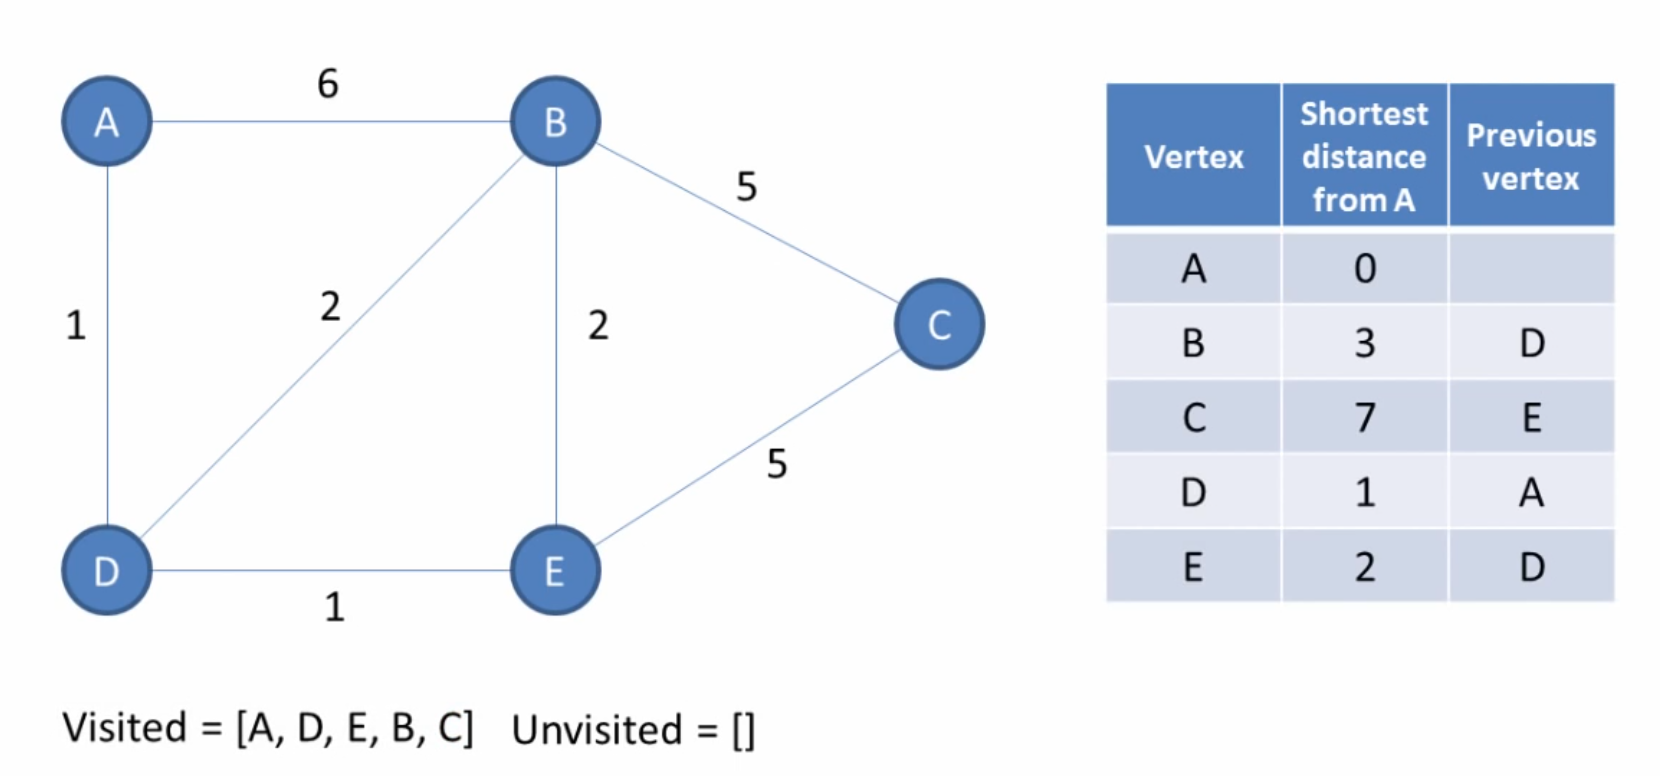
\includegraphics[width=15cm]{images/algo_dij}
  \caption{Exemple de calcul des plus courts chemins à partir du noeud A.}
  \label{fig:graph_dij}
\end{figure}

Sans entrer dans les détails d'implémentation que l'on trouve nombreux sur la toile et dans la littérature, l'algorithme de Dijkstra est 
un algorithme glouton qui utilise l'hypothèse qu'une décision prise sur la base
d'un critère d'optimalité locale conduira à un optimum global. Ainsi, à chaque itération, l'algorithme choisit, parmi les nœuds non traités, le nœud
du réseau dont la distance au nœud de départ est la plus faible. Après l'ajout de ce nœud au sous-graphe, on met à jour les distances des sommets voisins du nœud ajouté dans l'optique d'améliorer les chemins optimaux trouvés jusqu'ici. Généralement, on tient à jour une matrice et on remonte celle-ci à la fin de l'algorithme pour déterminer le chemin optimal entre deux sommets. Par exemple, sur la figure \ref{fig:graph_dij}, on voit que le plus court chemin pour aller de A à C a un coût de 7. On détermine ensuite de proche en proche le chemin le plus court grâce à la mémorisation des nœuds précédents. Ici, on voit que pour atteindre C avec le meilleur coût, on est passé par E, puis pour atteindre E, par D et en fin A. Le plus court chemin pour aller de A à C est donc ADEC. On utilise la même méthode pour déterminer tous les chemins optimaux 
d'origine A. Mais on peut n'avoir besoin que du calcul du chemin entre 2 sommets. De plus, la myopie de l'algorithme limite forcément ses performances. D'où l'idée
d'utiliser une heuristique visant à guider les choix locaux. Ce qui nous amène à l'algorithme A* présenté brièvement dans la suite.

% \begin{figure}[htp]
%   \centering
%   \tikzstyle{block} = [draw, fill=blue!20, rectangle, minimum height=3em, minimum width=6em, text width=6em,text centered]
\begin{tikzpicture}[auto, node distance=3.5cm,>=latex']
\shorthandoff{:} % Evite le bug de compilation avec tikz
    % Longueurs et espacement
    \def\longabove{0.2cm}
    \def\espacement{4cm}

    % Définition des blocs
    \node [block, node distance=\espacement] (codeur) {Codeur};
    \node [block, right of=codeur, node distance=\espacement] (cbs) {CBS};
    \node [block, right of=cbs, node distance=\espacement] (modulateur) {Modulateur};
 
    % Définition des liens
    \draw [<-] (codeur) -- ++(-2,0) node[left] {$\{b_n\}$};
    \draw [->] (codeur) -- node[above=\longabove] {$\{d_n\}$} (cbs);
    \draw [->] (cbs) -- node[above=\longabove] {$\{c_k\}$} (modulateur);
    \draw [->] (modulateur) -- ++(2,0) node[right] {$s(t)$};
\end{tikzpicture}

%   \caption{Exemple de diagramme TikZ.}
%   \label{fig:une-image}
% \end{figure}
\paragraph{Algorithme A* : }

A* est l'algorithme qu'on utilise intuitivement pour se déplacer d'un endroit à un autre dans une ville
connaissant la direction à prendre. Grâce à cette information supplémentaire, A* va privilégier le nœud qui minimise 
la somme de la distance déjà parcourue et de la distance estimée restant à parcourir, qui peut être ici la distance à vol d'oiseau.


Cet algorithme a été proposé pour la première fois 
par Peter E. Hart, Nils John Nilsson et Bertram Raphael
en 1968. Il s'agit d'une extension de l'algorithme de Dijkstra et s'applique comme ce dernier
à des graphes munis d'une distance positive. A* est très performant dans le cas où le graphe comporte une faible densité de nœuds 
mais n'est pas ou peu efficace dans le cas de parcours de labyrinthes par exemple.


Il faut tout d'abord choisir, en fonction du problème, une heuristique $h$, c'est-à-dire ici une fonction qui estime la distance 
restante entre chaque nœud et l'arrivée, estimation par défaut qui ne doit jamais surestimer cette distance. 
La précision du résultat final dépendra de la précision de l'estimation.
On peut citer les heuristiques suivantes : la distance euclidienne (norme 2) ou à ``vol d'oiseau'' déjà citée 
et la distance de Manhattan (norme 1) qui, sur une grille, correspond à la somme des cases verticales et horizontales
qui sépare la position courante de l'arrivée. Dans l'exemple du plan, les deux distances sont bien utilisables dans A* car elles sont des fonctions minorantes de la distance à l'arrivée.

À chaque étape l'algorithme calcule, pour chaque voisin non visité $n$ du point courant, la valeur $f(n) = g(n) + h(n)$ où $g(n)$ correspond au coût réel et minimal menant à $n$ et $h(n)$ la distance minorée qui relie $n$ à l'arrivée. L'exploration tient ainsi à jour une file, où les nœuds minimisant $f$ sont explorés en priorité. Lorsque l'heuristique est la fonction nulle, A* est équivalent à l'algorithme de Dijkstra.


\paragraph{Utilisation} L'application évidente de ces algorithmes dans le cadre du calcul parallèle est le transfert optimal de données d'un nœud \textit{A} vers un nœud \textit{B}. Cette application est d'ailleurs largement inspirée du domaine des réseaux de communication qui utilisent aussi la modélisation par graphes. On retrouve ainsi l'algorithme de Dijkstra dans le protocole de routage dynamique \textit{OSPF} qui est au cœur de l'interconnexion de réseaux et où les poids peuvent par exemple correspondre à la bande-passante des liens. Aujourd'hui, le \textit{cloud computing} qui vise à exploiter la puissance de calcul de machines distantes par l'intermédiaire d'un réseau, généralement Internet, fait donc un usage intensif de ces protocoles de routage. Quant à l'algorithme A*, si l'on souhaite exploiter tout son potentiel, il convient de définir une heuristique qui serait alors fonction de la topologie considérée.

\paragraph{} Enfin, notons que dans la plupart des cas, ces algorithmes n'ont de réelle utilité et d'existence qu'au niveau du réseau et des couches basses. En effet, au niveau logiciel, les topologies que nous présenterons, de par leur construction, permettent de développer très simplement des algorithmes de routage spécifiques (ce routage pourrait d'ailleurs se matérialiser sur un circuit intégré qui serait spécialement développé pour la topologie considérée).